%\vspace{-0.05in}
\section{Introduction}
%\vspace{-0.05in}
GPUs are now ubiquitous in systems ranging from mobile phones to datacenters like 
Amazon's elastic compute cloud (EC2) and HPC installations like Oak Ridge 
National Laboratory's Titan supercomputer.
%In all of these systems, GPUs are increasingly being used for processing beyond
%traditional computer graphics, including image processing, computer vision,
%machine learning, physical dynamics in games, and modeling high energy particle
%interactions. Regardless of the class of system being considered, GPU/CPU
%architectures are evolving towards general-purpose cache coherent non-uniform
%memory access (CC-NUMA) designs with both CPUs  and GPUs being able to access a
%unified globally-addressable memory~\cite{HSA}.  While some of these systems
%may share a single homogeneous pool of memory, an increasing number of systems
%use heterogeneous memory technologies.  Specifically, cost and/or energy
%concerns are driving memory system architects to provide a pool of
%high-bandwidth memory as well as a higher-capacity pool of lower-cost and/or
%lower-power memory.
Figure~\ref{fig:arch-asplos2015} shows several processor and memory topology options that
are likely to be common over the next several years. While traditional systems
are likely to continue using commodity DDR3 and soon DDR4, many future GPUs and
mobile systems are moving to also include higher bandwidth, but capacity
limited, on-package memories such as High Bandwidth Memory (HBM) or Wide-IO2
(WIO2)\@. Regardless the type of machine, both memories will be globally
accessible to maximize aggregate capacity and performance, making all systems
non-uniform memory access (NUMA) due to variations in latency, bandwidth, and
connection topology. Depending on the memories paired the bandwidth ratio
between the bandwidth-optimized (BO) and capacity or cost optimized (CO) memory
pools may be as low as 2$\times$ or as high as 8$\times$.

\begin{figure}[t]
    \centering
    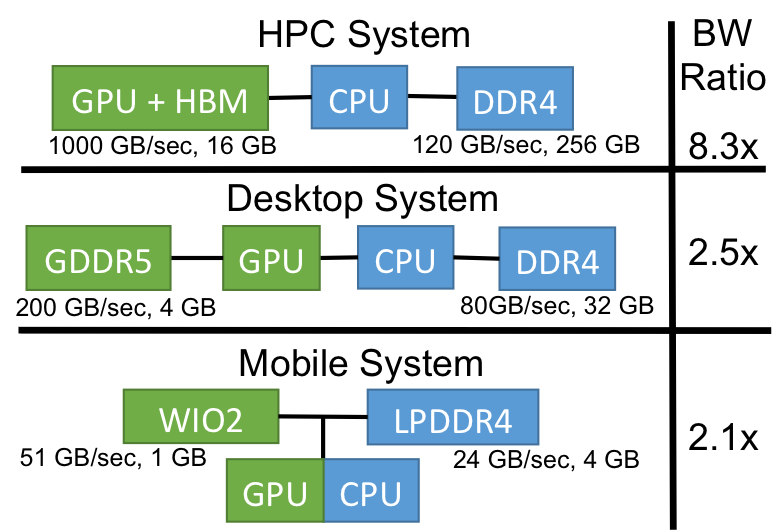
\includegraphics[width=0.8\columnwidth]{asplos2015/figures/arch}
    \caption{BW-Ratio of high-bandwidth vs high-capacity memories for likely future HPC, desktop, and mobile systems}
    \label{fig:arch-asplos2015}
\end{figure}

%To date, GPU-attached bandwidth optimized (BO) memory has been allocated and
%managed primarily as the result of explicit, programmer-directed function calls.
%As heterogeneous GPU/CPU systems move to a transparent unified memory system,
%the OS and runtime systems will become increasingly responsible for memory
%management functions such as page placement, just as they are in CPU-only NUMA
%systems today. In CC-NUMA systems, the notion of local versus remote memory
%latency is exposed to the operating system via the Advanced Configuration and
%Power Interface (ACPI). The latency differences between local and remote memory
%account for the additional latency incurred due to accessing remote memory
%across the system interconnect.  In these systems, latency information, alone,
%is adequate, as CPUs are generally more performance sensitive to memory system
%latency, rather than other memory characteristics.

Massively parallel GPUs and their highly-threaded programming models can
tolerate long memory latencies but, these throughput oriented processors demand
high bandwidth. However, due to lack of exposure of difference in bandwidth
capabilities differential of main memory technologies OS or the programmer, they
cannot make the best memory management decisions to exploit the memory bandwidth
of heterogeneous CPU-GPU system. In this thesis we explore the effect on GPU
performance of exposing memory system bandwidth information to the operating
system/runtime and user applications to improve the quality of dynamic page
placement decisions.

We explore two OS page placement policies:\\
1) Application agnostic Bandwidth-Aware (BW-AWARE) page placement policy that
can outperform Linux's current bandwidth-optimized INTERLEAVE placement by 35\%
and the default latency optimized LOCAL allocation policy by as much as 18\%,
when the application footprint fits within bandwidth-optimized memory capacity.  
\\
2) For \emph{memory capacity constrained} systems (i.e. bandwidth-optimized memory
capacity is insufficient for the workload footprint), we demonstrate that using
simple application annotations to inform the OS/runtime of hot versus
cold data structures can outperform the current Linux
INTERLEAVE and LOCAL page placement policies.  Our annotation
based policy combined with bandwidth information can outperform these
page placement policies by 19\% and 12\% respectively, and get within
90\% of oracle page placement performance.

%Contributions of this work include:
%
%\begin{enumerate}
%\item
%We show that existing CPU-oriented page placement policies are not only 
%sub-optimal for placement in GPU-based systems, but simply do not have the 
%appropriate information available to make informed decisions when optimizing for 
%bandwidth-asymmetric memory.  Exposing additional bandwidth information 
%to the OS, as is done for latency today, will be required for optimized decision 
%making.
%\item 
%Perhaps counter-intuitively we show that, placing all pages in the 
%bandwidth optimized memory is not the best performing page placement 
%policy for GPU workloads.  We propose and {\color{black}simulate} a new bandwidth-aware (BW-AWARE) page 
%placement policy that can outperform Linux's current bandwidth-optimized 
%INTERLEAVE placement by 35\% and the default latency optimized LOCAL allocation 
%policy by as much as 18\%, when the application footprint fits 
%within bandwidth-optimized memory capacity.  
%\item 
%For \emph{memory capacity constrained} systems (i.e. bandwidth-optimized memory
%capacity is insufficient for the workload footprint), we demonstrate that using
%simple application annotations to inform the OS/runtime of hot versus
%cold data structures can outperform the current Linux
%INTERLEAVE and LOCAL page placement policies.  Our annotation
%based policy combined with bandwidth information can outperform these
%page placement policies by 19\% and 12\% respectively, and get within
%90\% of oracle page placement performance.
%\end{enumerate}
